\subsection{The slab detachment}\label{sec:slab}
The slab detachment benchmark is performed as described by \citet{Schmalholz2011} and \citet{Glerum2018}. The domain is rectangular with $L_x=$ \SI{1000}{\km}
and $L_y=$ \SI{660}{\km} and a grid resolution of $256\times256$ elements. A non-linear viscous T-shaped layer with $\rho_l=$ \SI{3300}{\kg\per\cubic\metre} is
placed at the top of the domain and surrounded by a linear viscous fluid with $\rho_f=$ \SI{3150}{\kg\per\cubic\m}. The top layer is 80 km-thick and a 250
km-long and 80 km-wide slab is placed at $x=L_x/2$ (Fig. \ref{fig:slab}a).
\begin{figure}[h!]
\centering
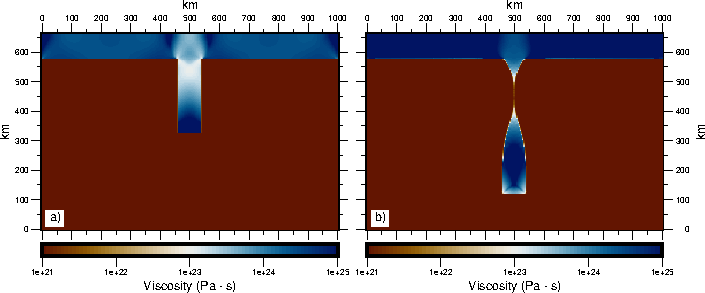
\includegraphics[width=14cm]{./Figures/Slab.pdf}
\caption{Effective viscosity for the slab detachment benchmark at the beginning of the evolution (panel a) and when necking is complete (panel b).}
\label{fig:slab}
\end{figure}

The effective viscosity of the top layer is given by
\begin{eqnarray}
\eta_{eff}=\eta_0 I_2^{\frac{(1-n)}{n}}\nonumber
\end{eqnarray}
with $\eta_0=$ \SI{4.75e11}{\pascal\s} and $n=4$, while the surrounding fluid has $\eta_f=$ \SI{e21}{\pascal\s}. The effective viscosity is capped between
$\eta_{min}=$ \SI{e21}{\pascal\s} and $\eta_{max}=$ \SI{e25}{\pascal\s}. Velocity boundary conditions are set to free slip at the top and the bottom, and to
no slip at the sides of the domain.

\begin{wrapfigure}{r}{11cm}
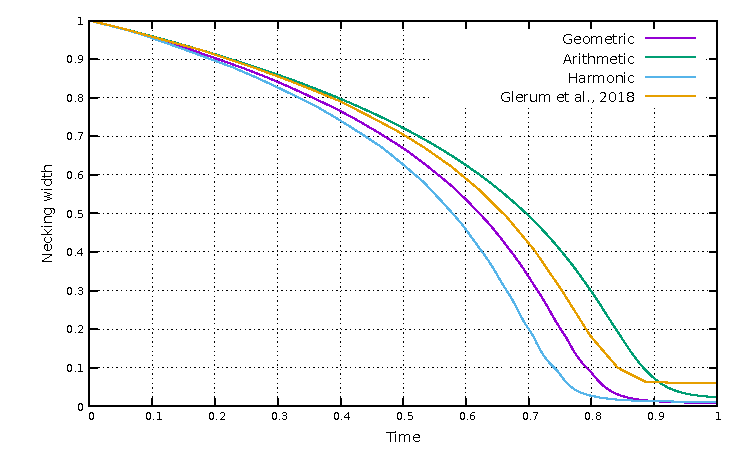
\includegraphics[width=11cm]{./Figures/Necking.pdf}
\caption{Normalised width of the necking of the slab detachment benchmark as function of normalised time.}
\label{fig:necking}
\end{wrapfigure}
The sinking of the slab determines a decrease of the effective viscosity in the T-shaped layer during the first part of the evolution (Fig. \ref{fig:slab}a),
as consequence of local strain rates, while effective viscosities increase up to $\eta_{max}$ in the top layer after approximately \SI{20}{\mega\year}, when
necking is complete (Fig. \ref{fig:slab}b).
The width of necking is tracked by means of markers position at the side of the slab. Necking width and time are normalised in function of the initial slab
(\SI{80}{\km}) and the characteristic time ($t_c=$ \SI{7.1158e14}{\s}) \citep{Schmalholz2011,Glerum2018}. The results in case of arithmetic, geometric and
harmonic mean of the viscosity are shown in Fig. \ref{fig:necking}, compared with results from \citet{Glerum2018} for which an infinity norm mean was used.
The influence of the average schemes agrees with results shown in Section \ref{sec:subduction}. All data can be 
found at \url{https://github.com/aleregorda/Benchmarks/tree/main/Nonlinear_visco_plasticity/Slab_detachment}.